% Options for packages loaded elsewhere
\PassOptionsToPackage{unicode}{hyperref}
\PassOptionsToPackage{hyphens}{url}
%
\documentclass[
]{book}
\usepackage{amsmath,amssymb}
\usepackage{iftex}
\ifPDFTeX
  \usepackage[T1]{fontenc}
  \usepackage[utf8]{inputenc}
  \usepackage{textcomp} % provide euro and other symbols
\else % if luatex or xetex
  \usepackage{unicode-math} % this also loads fontspec
  \defaultfontfeatures{Scale=MatchLowercase}
  \defaultfontfeatures[\rmfamily]{Ligatures=TeX,Scale=1}
\fi
\usepackage{lmodern}
\ifPDFTeX\else
  % xetex/luatex font selection
\fi
% Use upquote if available, for straight quotes in verbatim environments
\IfFileExists{upquote.sty}{\usepackage{upquote}}{}
\IfFileExists{microtype.sty}{% use microtype if available
  \usepackage[]{microtype}
  \UseMicrotypeSet[protrusion]{basicmath} % disable protrusion for tt fonts
}{}
\makeatletter
\@ifundefined{KOMAClassName}{% if non-KOMA class
  \IfFileExists{parskip.sty}{%
    \usepackage{parskip}
  }{% else
    \setlength{\parindent}{0pt}
    \setlength{\parskip}{6pt plus 2pt minus 1pt}}
}{% if KOMA class
  \KOMAoptions{parskip=half}}
\makeatother
\usepackage{xcolor}
\usepackage{color}
\usepackage{fancyvrb}
\newcommand{\VerbBar}{|}
\newcommand{\VERB}{\Verb[commandchars=\\\{\}]}
\DefineVerbatimEnvironment{Highlighting}{Verbatim}{commandchars=\\\{\}}
% Add ',fontsize=\small' for more characters per line
\usepackage{framed}
\definecolor{shadecolor}{RGB}{248,248,248}
\newenvironment{Shaded}{\begin{snugshade}}{\end{snugshade}}
\newcommand{\AlertTok}[1]{\textcolor[rgb]{0.94,0.16,0.16}{#1}}
\newcommand{\AnnotationTok}[1]{\textcolor[rgb]{0.56,0.35,0.01}{\textbf{\textit{#1}}}}
\newcommand{\AttributeTok}[1]{\textcolor[rgb]{0.13,0.29,0.53}{#1}}
\newcommand{\BaseNTok}[1]{\textcolor[rgb]{0.00,0.00,0.81}{#1}}
\newcommand{\BuiltInTok}[1]{#1}
\newcommand{\CharTok}[1]{\textcolor[rgb]{0.31,0.60,0.02}{#1}}
\newcommand{\CommentTok}[1]{\textcolor[rgb]{0.56,0.35,0.01}{\textit{#1}}}
\newcommand{\CommentVarTok}[1]{\textcolor[rgb]{0.56,0.35,0.01}{\textbf{\textit{#1}}}}
\newcommand{\ConstantTok}[1]{\textcolor[rgb]{0.56,0.35,0.01}{#1}}
\newcommand{\ControlFlowTok}[1]{\textcolor[rgb]{0.13,0.29,0.53}{\textbf{#1}}}
\newcommand{\DataTypeTok}[1]{\textcolor[rgb]{0.13,0.29,0.53}{#1}}
\newcommand{\DecValTok}[1]{\textcolor[rgb]{0.00,0.00,0.81}{#1}}
\newcommand{\DocumentationTok}[1]{\textcolor[rgb]{0.56,0.35,0.01}{\textbf{\textit{#1}}}}
\newcommand{\ErrorTok}[1]{\textcolor[rgb]{0.64,0.00,0.00}{\textbf{#1}}}
\newcommand{\ExtensionTok}[1]{#1}
\newcommand{\FloatTok}[1]{\textcolor[rgb]{0.00,0.00,0.81}{#1}}
\newcommand{\FunctionTok}[1]{\textcolor[rgb]{0.13,0.29,0.53}{\textbf{#1}}}
\newcommand{\ImportTok}[1]{#1}
\newcommand{\InformationTok}[1]{\textcolor[rgb]{0.56,0.35,0.01}{\textbf{\textit{#1}}}}
\newcommand{\KeywordTok}[1]{\textcolor[rgb]{0.13,0.29,0.53}{\textbf{#1}}}
\newcommand{\NormalTok}[1]{#1}
\newcommand{\OperatorTok}[1]{\textcolor[rgb]{0.81,0.36,0.00}{\textbf{#1}}}
\newcommand{\OtherTok}[1]{\textcolor[rgb]{0.56,0.35,0.01}{#1}}
\newcommand{\PreprocessorTok}[1]{\textcolor[rgb]{0.56,0.35,0.01}{\textit{#1}}}
\newcommand{\RegionMarkerTok}[1]{#1}
\newcommand{\SpecialCharTok}[1]{\textcolor[rgb]{0.81,0.36,0.00}{\textbf{#1}}}
\newcommand{\SpecialStringTok}[1]{\textcolor[rgb]{0.31,0.60,0.02}{#1}}
\newcommand{\StringTok}[1]{\textcolor[rgb]{0.31,0.60,0.02}{#1}}
\newcommand{\VariableTok}[1]{\textcolor[rgb]{0.00,0.00,0.00}{#1}}
\newcommand{\VerbatimStringTok}[1]{\textcolor[rgb]{0.31,0.60,0.02}{#1}}
\newcommand{\WarningTok}[1]{\textcolor[rgb]{0.56,0.35,0.01}{\textbf{\textit{#1}}}}
\usepackage{longtable,booktabs,array}
\usepackage{calc} % for calculating minipage widths
% Correct order of tables after \paragraph or \subparagraph
\usepackage{etoolbox}
\makeatletter
\patchcmd\longtable{\par}{\if@noskipsec\mbox{}\fi\par}{}{}
\makeatother
% Allow footnotes in longtable head/foot
\IfFileExists{footnotehyper.sty}{\usepackage{footnotehyper}}{\usepackage{footnote}}
\makesavenoteenv{longtable}
\usepackage{graphicx}
\makeatletter
\def\maxwidth{\ifdim\Gin@nat@width>\linewidth\linewidth\else\Gin@nat@width\fi}
\def\maxheight{\ifdim\Gin@nat@height>\textheight\textheight\else\Gin@nat@height\fi}
\makeatother
% Scale images if necessary, so that they will not overflow the page
% margins by default, and it is still possible to overwrite the defaults
% using explicit options in \includegraphics[width, height, ...]{}
\setkeys{Gin}{width=\maxwidth,height=\maxheight,keepaspectratio}
% Set default figure placement to htbp
\makeatletter
\def\fps@figure{htbp}
\makeatother
\setlength{\emergencystretch}{3em} % prevent overfull lines
\providecommand{\tightlist}{%
  \setlength{\itemsep}{0pt}\setlength{\parskip}{0pt}}
\setcounter{secnumdepth}{5}
\ifLuaTeX
  \usepackage{selnolig}  % disable illegal ligatures
\fi
\usepackage[]{natbib}
\bibliographystyle{apalike}
\IfFileExists{bookmark.sty}{\usepackage{bookmark}}{\usepackage{hyperref}}
\IfFileExists{xurl.sty}{\usepackage{xurl}}{} % add URL line breaks if available
\urlstyle{same}
\hypersetup{
  pdftitle={Study Note for 24Q2 AppFin704},
  pdfauthor={Author: Jung Xue},
  hidelinks,
  pdfcreator={LaTeX via pandoc}}

\title{Study Note for 24Q2 AppFin704}
\author{Author: Jung Xue}
\date{Last Updated: 2024-05-26}

\begin{document}
\maketitle

{
\setcounter{tocdepth}{1}
\tableofcontents
}
\hypertarget{ch1}{%
\chapter{Investments and Securities Markets}\label{ch1}}

•describe differences among asset classes and construction of stock market indexes, and calculate profit/loss on options/futures investments.

•describe how firms issue securities, and identify types of investors' orders

•compare mechanics and implications of buying on margin \& short selling

•cite pros/cons of investing with an investment company, and contrast open end mutual funds with other types of investment companies.

•define net asset value (NAV) and measure the rate of return on a mutual fund, and classify mutual funds according to investment style.

•demonstrate the impact of expenses and turnover on fund performance

\hypertarget{asset-classes-and-financial-instruments}{%
\section{Asset Classes and Financial Instruments}\label{asset-classes-and-financial-instruments}}

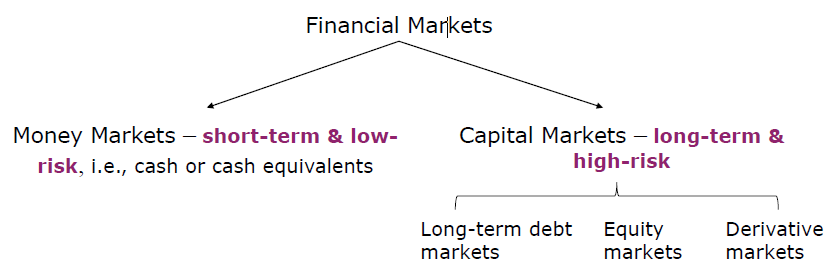
\includegraphics{Resources/Financialmarkets.png}

\hypertarget{money-markets}{%
\subsection{Money Markets}\label{money-markets}}

\begin{itemize}
\tightlist
\item
  Treasury bills
\item
  Certificates of Deposits (Term Deposits)
\item
  Commercial Paper(CP) (short term \textless{} 12month unsecured debts)
\item
  Bankers Acceptances (a postdated check, A bank, rather than an account holder, guarantees the payment.)
\item
  Eurodollars (U.S. dollar denominated deposits at foreign banks or foreign branches of U.S. banks)
\item
  Repurchase Agreements (Repos or RPs) and Reverse Repos.
\item
  Others, e.g., Brokers' Calls (interests charged by banks on loans made to brokerage firms), Federal Funds, The LIBOR Market, and Money Market Funds
\end{itemize}

\hypertarget{the-bond-market}{%
\subsection{The Bond Market}\label{the-bond-market}}

\begin{itemize}
\tightlist
\item
  Treasury Notes/Bonds (\$21 billion, \$21/\$51= 41\% of 2020 US Bond Market)
\item
  Mortgages and Mortgage Backed Securities (\$12.7 billion, 25\%
\item
  Corporate Bonds, including secured bonds, debentures (unsecured), callable/puttable/convertible bonds (\$10.6 billion, 21\%
\item
  Municipal Bonds (Issued by states/local, tax exempt) (\$3.95 billion, 7.8\%)
\item
  Federal Agency Debt, e.g., Fannie Mae, Freddie Mac ( 3.3\%)
\item
  International Bonds

  \begin{itemize}
  \tightlist
  \item
    Eurobonds: Eurodollar bonds bonds denominated in a currency other than the issuer's currency
  \item
    Yankee bond: US dollar denominated bond sold in the U.S. by a non U.S. issuer
  \end{itemize}
\item
  Inflation Protected Bonds (i.e., principal is adjusted per CPI)
\end{itemize}

\hypertarget{the-equity-market}{%
\subsection{The Equity Market}\label{the-equity-market}}

\begin{itemize}
\tightlist
\item
  Common stocks
\item
  Preferred stocks (pay preferred dividends, behaving like bond)
\item
  Depository receipts, (shares in a foreign company)

  \begin{itemize}
  \tightlist
  \item
    ADR American Depository Receipt
  \item
    CRD Chinese Depository receipt
  \item
    Reduced currency and foreign operation cost
  \end{itemize}
\end{itemize}

\hypertarget{market-indexes}{%
\subsection{Market Indexes}\label{market-indexes}}

\begin{itemize}
\tightlist
\item
  Broad based index (S\&P 500 etc.)
\item
  Narrow based index (composed of only a few stocks, in a specific industry)
\item
  Why indexes?
\item
  Provide performance benchmarks
\item
  Base of derivatives
\item
  Smart beta
\end{itemize}

The goal of \textbf{Smart beta} is to obtain alpha, lower risk or increase diversification at a cost lower than traditional active management and marginally higher than straight index investing

Construction Methodology

\begin{itemize}
\tightlist
\item
  Price weighted (DJIA) 1 share per firm
\item
  Market value weighted (S\&P500, NASDAQ)
\item
  Equal weighted (simple average of returns)
\end{itemize}

\hypertarget{derivative-markets}{%
\subsection{Derivative Markets}\label{derivative-markets}}

\begin{itemize}
\tightlist
\item
  A security with a pay-off that depends on the prices of other securities
\item
  Call/put options
\item
  Futures/Forwards
\item
  Swaps, futures options, etc.
\end{itemize}

Why we need them?

\begin{itemize}
\tightlist
\item
  Speculative
\item
  Hedging
\item
  Arbitraging (to lock in price)
\end{itemize}

\textbf{Arbitrage} describes the act of buying a security in one market and simultaneously selling it in another market at a higher price, thereby enabling investors to profit from the temporary difference in cost per share.

\hypertarget{securities-markets-and-trading}{%
\section{Securities Markets and Trading}\label{securities-markets-and-trading}}

Originators

\begin{itemize}
\tightlist
\item
  Publicly traded companies initial public offering (IPO), and seasonal equity offerings (SEOs), - Privately held firms (private placement in which shares are sold directly to
  a small group of institutional or wealthy investors)
\item
  Shelf registrations (public firms can register securities and gradually sell them to the public )
\end{itemize}

How securities are traded (in secondary markets)

\begin{itemize}
\tightlist
\item
  Direct search (e.g.~painting)
\item
  Brokered
\item
  Dealer
\item
  Auctions
\end{itemize}

ype of orders
maket order
price contingeant order

Trading mechanisms
OTC dealer
electronic
market maker (increase liquidity)
--
Over the counter dealer markets (OTC Markets)
-
Electronic communication networks ( ECNs)

margin trading

why to purchase with margin?

able to make more profits by borrowing money from broker, essentially multiplying market fluctuation/volatility.

short sale (borrow stocks to sell and payback when you sold it at profit)

derivative market (sell, not borrowing)

\hypertarget{market-participants}{%
\section{Market Participants}\label{market-participants}}

\hypertarget{investment-company}{%
\subsection{Investment company}\label{investment-company}}

\begin{itemize}
\tightlist
\item
  Intermediary that invest for investors
\item
  Record and admin
\item
  professional management
\item
  Lower transaction cost by volume
\end{itemize}

Net Asset Value (NAV)

\[\frac{Asset - Liabilities}{share outstanding}\]
unit investement fund (unmanaged) fixed portfolio for life

Managed Investment companies
- open-end(publicly trader and closed ended)
- close end funds shares sold at discount for liquidity (to sell quickly)

Exchange Traded Funds (ETF)

Can be continuously traded like stocks

Other Comingled Funds, Real Estate Investment Trusts, Hedged Funds

Mutual Funds 65\% of market

\begin{itemize}
\tightlist
\item
  Money market
\item
  equity funds (income vs growth)
\item
  specialised
\item
  bond
\item
  index funds
\item
  Funds of Funds
\end{itemize}

Funds can be sold directly, indirectly and through financial supermarkets

Fee structure

\begin{itemize}
\tightlist
\item
  Operating expense
\item
  front end load
\item
  back end load
\item
  12b-1 charges annual fee fro marketing and distribution
\end{itemize}

fee structure is very important and made large apart of your profit share

Taxation

no tax at fund level
long term capital gain tax rate
high turnover rate

ETF
- Passive investement, track index
- lower cost
- smart beta fund

\begin{itemize}
\tightlist
\item
  Bid ask spread (depend on demand)
\item
  Index price depart from NAV
\end{itemize}

mutual fund underperformed passive funds(cost of high freq trading)

consistent performance, don't be obsessed with top performer, they could be winner by chance

\hypertarget{ch2}{%
\chapter{Risk and Return}\label{ch2}}

\hypertarget{learning-objectives}{%
\section{Learning Objectives}\label{learning-objectives}}

This lecture aims to provide the ability to:

\begin{enumerate}
\def\labelenumi{\arabic{enumi}.}
\tightlist
\item
  Compute various measures of return on multi-year investments.
\item
  Determine the expected return and risk of portfolios combining risky assets and risk-free investments like Treasury bills.
\item
  Use the \textbf{Sharpe ratio} for evaluating portfolio performance and guiding capital allocation.
\item
  Understand the role of utility in determining optimal capital allocation to risky assets.
\end{enumerate}

\hypertarget{measuring-returns}{%
\section{Measuring Returns}\label{measuring-returns}}

Returns can be measured in several ways:

\begin{itemize}
\tightlist
\item
  \textbf{Holding Period Return (HPR):} This is the return earned over the period an investment is held.
\item
  \textbf{Returns Over Multiple Periods:} These can be compounded over time using methods such as:

  \begin{itemize}
  \tightlist
  \item
    arithmetic average,
  \item
    geometric average (compound annual growth rate), and
  \item
    dollar-weighted average (internal rate of return).
  \end{itemize}
\end{itemize}

\hypertarget{arithmetic-average}{%
\subsection{Arithmetic Average}\label{arithmetic-average}}

\[ \text{Arithmetic Average} = \frac{1}{N} \sum_{i=1}^{N} r_i \]
where \(r_i\) is the return in period \(i\) and \(N\) is the total number of periods.

\hypertarget{geometric-average}{%
\subsection{Geometric Average}\label{geometric-average}}

\[ \text{Geometric Average} = \left( \prod_{i=1}^{N} (1 + r_i) \right)^{\frac{1}{N}} - 1 \]

where \(r_i\) is the return in period \(i\) and \(N\) is the total number of periods.

\hypertarget{dollar-weighted-average-internal-rate-of-return}{%
\subsection{Dollar-Weighted Average (Internal Rate of Return)}\label{dollar-weighted-average-internal-rate-of-return}}

The dollar-weighted average return, or internal rate of return (IRR), is the discount rate \(r\) that sets the \textbf{net present value (NPV) = 0}. It is calculated by solving the following equation:

\[ \text{Dollar-Weighted Average} = \sum_{t=0}^{N} \frac{C_t}{(1 + r)^t} = 0 \]

Where \(C_t\) is the net cash flow at time \(t\), and \(N\) is the total number of periods.

\hypertarget{annualizing-returns}{%
\subsection{Annualizing Returns}\label{annualizing-returns}}

\begin{itemize}
\tightlist
\item
  \textbf{Annual Percentage Rate (APR):} Simple annualized interest rate without compounding.
\item
  \textbf{Effective Annual Rate (EAR):} Accounts for intra-year compounding, providing a true measure of annual return.
\end{itemize}

\[
\text{APR} = r \times n
\]

Where:

\begin{itemize}
\tightlist
\item
  \(r\) is the periodic interest rate
\item
  \(n\) is the number of compounding periods per year
\end{itemize}

\[
\text{EAR} = \left(1 + \frac{r}{n}\right)^n - 1
\]
Where:

\begin{itemize}
\tightlist
\item
  \(r\) is the nominal annual interest rate
\item
  \(n\) is the number of compounding periods per year
\end{itemize}

Example:

\$ 10000 Deposit, APR (annual percentage rate): 4\% p.a. Compounding Quarterly.

\[ 
\begin{aligned}
EAR &= (1+r/n)^n− 1 \\
&=(1+(0.04)/4)^4 −1 \\
&=0.0406 \\
&= 4.06\% 
\end{aligned}
\]

\hypertarget{risk-and-risk-premiums}{%
\section{Risk and Risk Premiums}\label{risk-and-risk-premiums}}

\hypertarget{expected-return}{%
\subsection{Expected Return}\label{expected-return}}

\(E(R)\) Is the weighted average of all possible returns, with weights being the probabilities of each scenario.

\[
E(R) = \sum_{i=1}^{N} p_i \cdot r_i
\]
Where:

\begin{itemize}
\tightlist
\item
  \(E(R)\) is the expected return of the portfolio
\item
  \(p_i\) is the probability/weight of asset \(i\) in the portfolio
\item
  \(r_i\) is the expected return of individual asset \(i\)
\item
  \(N\) is the number of assets in the portfolio
\end{itemize}

\textbf{Example Calculation}

\begin{itemize}
\tightlist
\item
  Asset A: weight = 50\%, expected return = 10\%
\item
  Asset B: weight = 30\%, expected return = 15\%
\item
  Asset C: weight = 20\%, expected return = 20\%
\end{itemize}

The expected return of the portfolio is:

\[
\begin{aligned}
E(R) &= (0.50 \cdot 0.10) + (0.30 \cdot 0.15) + (0.20 \cdot 0.20) \\
       &= 0.05 + 0.045 + 0.04 \\
       &= 0.135 \\
       &= 13.5\% \\  
\end{aligned}
\]
\textbf{R Code for Calculation}

\begin{Shaded}
\begin{Highlighting}[]
\CommentTok{\# Define the weights and expected returns of the assets}
\NormalTok{weights          }\OtherTok{\textless{}{-}} \FunctionTok{c}\NormalTok{(}\FloatTok{0.50}\NormalTok{, }\FloatTok{0.30}\NormalTok{, }\FloatTok{0.20}\NormalTok{)}
\NormalTok{expected\_returns }\OtherTok{\textless{}{-}} \FunctionTok{c}\NormalTok{(}\FloatTok{0.10}\NormalTok{, }\FloatTok{0.15}\NormalTok{, }\FloatTok{0.20}\NormalTok{)}

\CommentTok{\# Calculate the expected return of the portfolio}
\NormalTok{expected\_return\_portfolio }\OtherTok{\textless{}{-}} \FunctionTok{sum}\NormalTok{(weights }\SpecialCharTok{*}\NormalTok{ expected\_returns)}

\CommentTok{\# Print the expected return as a percentage}
\NormalTok{expected\_return\_percentage }\OtherTok{\textless{}{-}}\NormalTok{ expected\_return\_portfolio }\SpecialCharTok{*} \DecValTok{100}
\NormalTok{expected\_return\_percentage}
\end{Highlighting}
\end{Shaded}

\begin{verbatim}
## [1] 13.5
\end{verbatim}

\hypertarget{standard-deviation}{%
\subsection{Standard Deviation}\label{standard-deviation}}

Measures the deviation of returns from the mean.

\[
\sigma = \sqrt{\sum_{i=1}^{N} p(i) [r(i) - E(r)]^2}
\]

Where:

\begin{itemize}
\tightlist
\item
  \(\sigma\) is the standard deviation of the expected return
\item
  \(p(i)\) is the probability/weight of assets \(i\)
\item
  \(r(i)\) is the return of individual assets \(i\)
\item
  \(E(r)\) is the expected return
\item
  \(N\) is the number of assets
\end{itemize}

\textbf{Example Calculation}

\begin{itemize}
\tightlist
\item
  asset 1: probability = 0.3, return = 0.12
\item
  asset 2: probability = 0.4, return = 0.04
\item
  asset 3: probability = 0.3, return = -0.02
\item
  Expected return \(E(r) = 0.046\)
\end{itemize}

The standard deviation of the expected return is:

\[
\begin{aligned}
\sigma &= \sqrt{0.3(0.12 - 0.046)^2 + 0.4(0.04 - 0.046)^2 + 0.3(-0.02 - 0.046)^2}\\
       &= 0.0544\\
       &= 5.44\%
\end{aligned}
\]
\textbf{R Code for Calculation}

\begin{Shaded}
\begin{Highlighting}[]
\CommentTok{\# Define the probabilities and returns of the states}
\NormalTok{probabilities }\OtherTok{\textless{}{-}} \FunctionTok{c}\NormalTok{(}\FloatTok{0.3}\NormalTok{, }\FloatTok{0.4}\NormalTok{, }\FloatTok{0.3}\NormalTok{)}
\NormalTok{returns }\OtherTok{\textless{}{-}} \FunctionTok{c}\NormalTok{(}\FloatTok{0.12}\NormalTok{, }\FloatTok{0.04}\NormalTok{, }\SpecialCharTok{{-}}\FloatTok{0.02}\NormalTok{)}
\NormalTok{expected\_return }\OtherTok{\textless{}{-}} \FloatTok{0.046}

\CommentTok{\# Calculate the variance}
\NormalTok{variance }\OtherTok{\textless{}{-}} \FunctionTok{sum}\NormalTok{(probabilities }\SpecialCharTok{*}\NormalTok{ (returns }\SpecialCharTok{{-}}\NormalTok{ expected\_return)}\SpecialCharTok{\^{}}\DecValTok{2}\NormalTok{)}

\CommentTok{\# Calculate the standard deviation}
\NormalTok{standard\_deviation }\OtherTok{\textless{}{-}} \FunctionTok{sqrt}\NormalTok{(variance)}

\CommentTok{\# Print the standard deviation as a percentage}
\NormalTok{standard\_deviation\_percentage }\OtherTok{\textless{}{-}}\NormalTok{ standard\_deviation }\SpecialCharTok{*} \DecValTok{100}
\NormalTok{standard\_deviation\_percentage}
\end{Highlighting}
\end{Shaded}

\begin{verbatim}
## [1] 5.444263
\end{verbatim}

\hypertarget{normal-distribution}{%
\subsection{Normal Distribution}\label{normal-distribution}}

Stock returns are often assumed to be normally distributed. However, real return distributions may show skewness such as ``fat tails.''

\[X∼N(μ,σ2)\]

\[
f(x | \mu, \sigma) = \frac{1}{\sigma \sqrt{2\pi}} \exp\left(-\frac{(x - \mu)^2}{2\sigma^2}\right)
\]

Where:

\begin{itemize}
\tightlist
\item
  \(\mu\) is the mean
\item
  \(\sigma\) is the standard deviation
\item
  \(x\) is the variable
\end{itemize}

\textbf{standard normal distribution} is the normal distribution with mean \(μ\) = 0 and standard deviation \(σ\) = 1.

\[
f(x) = \frac{1}{\sqrt{2\pi}} \exp\left(-\frac{x^2}{2}\right)
\]

Where:

\begin{itemize}
\tightlist
\item
  \(\mu = 0\)
\item
  \(\sigma = 1\)
\item
  \(x\) is the variable
\end{itemize}

\textbf{Example Calculation}

Let's calculate the probability of a value \(x\) in a normal distribution with a mean \(\mu = 0\) and a standard deviation \(\sigma = 1\) (standard normal distribution).

We will also calculate the cumulative probability (CDF) and quantiles for specific values.

\textbf{R Code for Calculation}

\begin{Shaded}
\begin{Highlighting}[]
\CommentTok{\# Define the parameters for the normal distribution}
\NormalTok{mu }\OtherTok{\textless{}{-}} \DecValTok{0}
\NormalTok{sigma }\OtherTok{\textless{}{-}} \DecValTok{1}

\CommentTok{\# Define a value for x}
\NormalTok{x }\OtherTok{\textless{}{-}} \DecValTok{1}

\CommentTok{\# Calculate the probability density function (PDF) of the normal distribution at x}
\NormalTok{pdf\_value }\OtherTok{\textless{}{-}} \FunctionTok{dnorm}\NormalTok{(x, }\AttributeTok{mean =}\NormalTok{ mu, }\AttributeTok{sd =}\NormalTok{ sigma)}

\CommentTok{\# Calculate the cumulative distribution function (CDF) of the normal distribution at x}
\NormalTok{cdf\_value }\OtherTok{\textless{}{-}} \FunctionTok{pnorm}\NormalTok{(x, }\AttributeTok{mean =}\NormalTok{ mu, }\AttributeTok{sd =}\NormalTok{ sigma)}

\CommentTok{\# Calculate the quantile for a given probability}
\NormalTok{probability }\OtherTok{\textless{}{-}} \FloatTok{0.95}
\NormalTok{quantile\_value }\OtherTok{\textless{}{-}} \FunctionTok{qnorm}\NormalTok{(probability, }\AttributeTok{mean =}\NormalTok{ mu, }\AttributeTok{sd =}\NormalTok{ sigma)}

\CommentTok{\# Print the results}
\FunctionTok{list}\NormalTok{(}\AttributeTok{PDF =}\NormalTok{ pdf\_value, }\AttributeTok{CDF =}\NormalTok{ cdf\_value, }\AttributeTok{Quantile =}\NormalTok{ quantile\_value)}
\end{Highlighting}
\end{Shaded}

\begin{verbatim}
## $PDF
## [1] 0.2419707
## 
## $CDF
## [1] 0.8413447
## 
## $Quantile
## [1] 1.644854
\end{verbatim}

\hypertarget{risk-aversion}{%
\subsection{Risk Aversion}\label{risk-aversion}}

Risk-averse investors prefer less risk for the same expected return. They demand a risk premium for taking additional risk, quantified by the price of risk (ratio of risk premium to variance).

Risk-averse investors reject investment opportunities with a \textbf{risk premium} of zero or less.

\textbf{Degree of risk aversion}

\[
A = \frac{E(r_i) - E(r_f)}{\sigma_i^2}
\]

Where:

\begin{itemize}
\tightlist
\item
  \(A\) = degree of risk aversion
\item
  \(E(r_i)\) is the expected return of the risky asset.
\item
  \(E(r_f)\) is the risk-free rate.
\item
  \(\sigma_i^2\) is the variance of the return of the risky asset.
\end{itemize}

\textbf{Example}

For the market portfolio (e.g., S\&P 500 index funds), the average degree of risk aversion of investors is:

\[
\begin{aligned}
\bar{A} &= \frac{\text{Average}(r_M - r_f)}{\text{Sample } \sigma_M^2}\\
 &\approx \frac{0.08}{0.04} = 2
\end{aligned}
\]

Where:

\begin{itemize}
\tightlist
\item
  \(r_M\) is the return of the market portfolio.
\item
  \(\sigma_M^2\) is the variance of the market return.
\end{itemize}

\hypertarget{portfolio-construction}{%
\section{Portfolio Construction}\label{portfolio-construction}}

\begin{enumerate}
\def\labelenumi{\arabic{enumi}.}
\item
  Selection of risky assets/portfolios such as stocks and bonds.
\item
  Decision on the proportion of the portfolio to invest in risky assets versus risk-free assets.
\end{enumerate}

\hypertarget{capital-allocation}{%
\subsection{Capital Allocation:}\label{capital-allocation}}

Combining investments in risk-free and risky assets allows for varying expected returns and risks.

We call the overall portfolio composed of the risk-free asset and the risky portfolio the \textbf{complete portfolio}.

\hypertarget{utility}{%
\subsection{Utility}\label{utility}}

\textbf{Utility:} Represents investor preferences, considering risk aversion. It helps in making decisions about different securities.This is a single measure we have the investor's attitudes to risk and return at each level of wealth.

\textbf{Influence of the trade-off decisions:}

\begin{itemize}
\tightlist
\item
  Risk appetite (strong financial position and stable income may have higher appitite)
\item
  proportion of the investor's total wealth. (psychological risk aversion)
\item
  Financial Goals/liquidity needs (set when they need cash flow)
\item
  Investment Horizon (longer horizon takes more risk)
\item
  Knowledge and Experience (Dunning Kruger effect)
\item
  Social/Regulatory environment and incentives
\end{itemize}

\hypertarget{utility-function}{%
\subsection{Utility Function}\label{utility-function}}

Captures an investor's risk-return trade-offs. Utility increases with expected return and decreases with risk. More risk-averse investors have higher coefficients of risk aversion (A).

There are countless utility functions. An example is:

\[
U = E(r) - \frac{1}{2} A \sigma^2
\]
Where:

\begin{itemize}
\tightlist
\item
  \(U\) = the utility value,
\item
  \(A\) = coefficient of risk aversion,
\item
  \(\sigma^2\) = variance
\item
  Utility increases with expected returns and decreases with risk.
\item
  Utility of a risk-free portfolio is equal to its rate of return.
\item
  More risk-averse investors will have larger values of A.
\item
  Investors assign higher utility to more attractive risk-return portfolios.
\end{itemize}

\textbf{Example:}

where:

\begin{itemize}
\tightlist
\item
  \(A\) degree of risk aversion = \(2\)
\item
  \(r_f\) risk-free rate = \(4\%\)
\end{itemize}

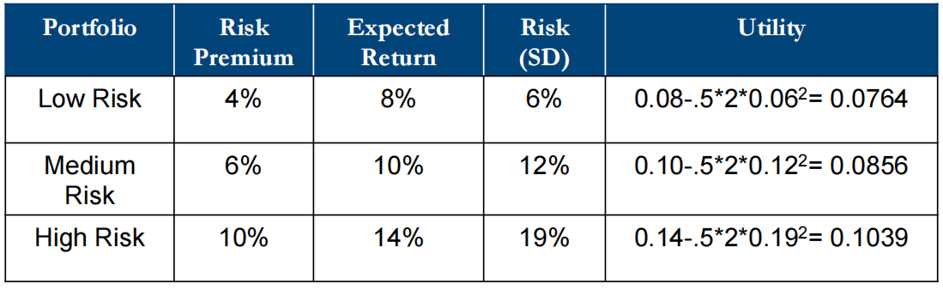
\includegraphics{Resources/utilisation.png}

\hypertarget{indifference-curves}{%
\subsection{Indifference Curves}\label{indifference-curves}}

These curves connect portfolios providing the same utility level, illustrating an investor's preference for different risk-return combinations.

Simply above the curve Yes, below the curve no.

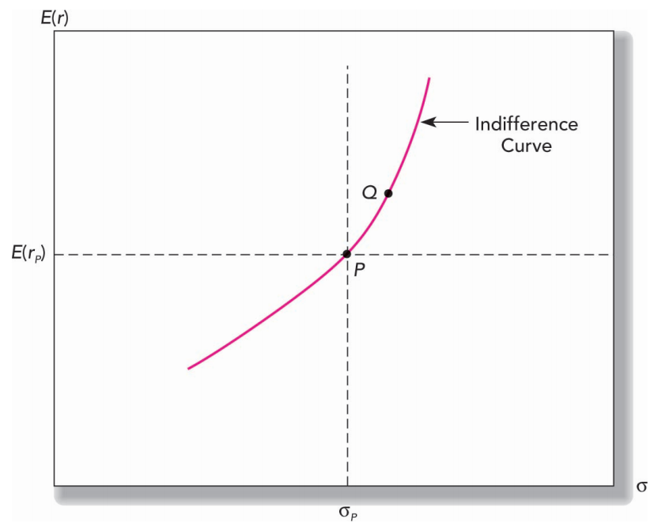
\includegraphics{Resources/indiffcurve.png}

\hypertarget{capital-allocation-line}{%
\subsection{Capital Allocation Line}\label{capital-allocation-line}}

It's possible to split investment funds between safe and risky assets.

\begin{enumerate}
\def\labelenumi{\arabic{enumi}.}
\tightlist
\item
  Risk free asset: proxy = T-bills
\item
  Risky asset: stock (or a portfolio)
\end{enumerate}

\begin{itemize}
\tightlist
\item
  \(r_f\) Risk-free rate = \(7\%\)
\item
  \(\sigma_{r_f}\) Standard deviation of the risk-free rate = \(0\)
\item
  \(E(r_p)\) Expected return of the risky portfolio = \(15\%\)
\item
  \(\sigma_p\) Standard deviation of the risky portfolio = \(22\%\)
\end{itemize}

The investor allocates \(y\) proportion of their wealth in the risky portfolio and \(1 - y\) in the risk-free portfolio.

\[
\begin{aligned}
E(r_c) &= (y)E(r_p) + (1 - y)r_f \\
E(r_c) &= y \times 15\% + (1 - y) \times 7\% \\
E(r_c) &= 7\% + y \times (15\% - 7\%) \\
E(r_c) &= 7\% + 8y \\
and \\
\sigma_c &= y \sigma_𝑝=22𝑦\\
\end{aligned}
\]

Example:

\[
\begin{aligned}
y        &= 0.75 \\
r_𝑐     &= 0.07+0.08*(0.75) = 13\% \\
\sigma_c &= y \sigma_𝑝=22𝑦\\
\sigma_c &= 16.5\% \\
\end{aligned}
\]
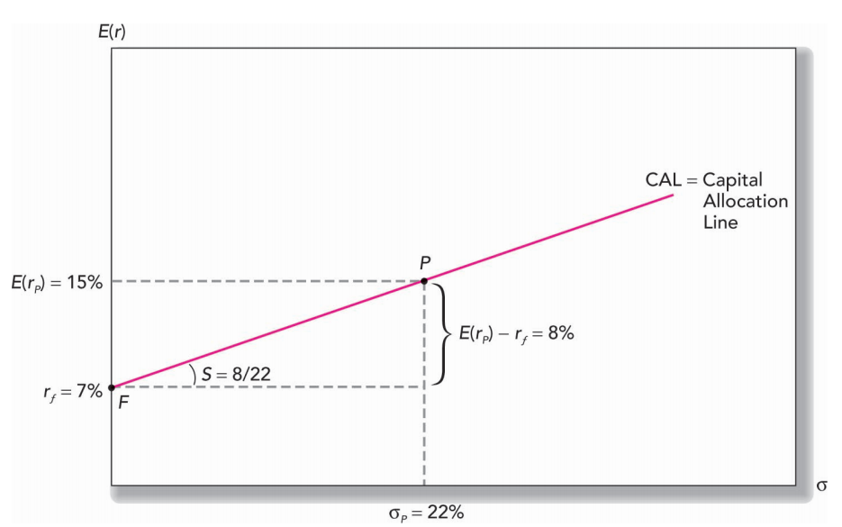
\includegraphics{Resources/capaloocation1.png}

The \textbf{Sharpe Ratio}, which measures extra return per unit of risk (gradient of line), is calculated as:

\[
\begin{aligned}
\text{Sharpe ratio} &= \frac{E(r_p) - r_f}{ \sigma_p}\\
&= 8/22 \\
&= 0.36\%. 
\end{aligned}
\]

\hypertarget{capital-allocation-line-cal-with-leverage}{%
\subsection{Capital Allocation Line (CAL) with Leverage}\label{capital-allocation-line-cal-with-leverage}}

Leverage multiplies loss and return at a cost of borrowing money from dealers.

Borrowing at the risk-free rate extends the CAL. Borrowing rates higher than the risk-free rate cause a kink in the CAL, changing the slope.

\[
\begin{aligned}
      𝐸(r_c) &= (−0.5)∗0.09+(1.5)∗0.15\\
              &=18\% \\
       \sigma_c &= (1.5)0.22 = 33\% \\
\text{The Sharpe ratio is} \\
    (18−9)/0.33 &= 0.27\% \\
\end{aligned}
\]
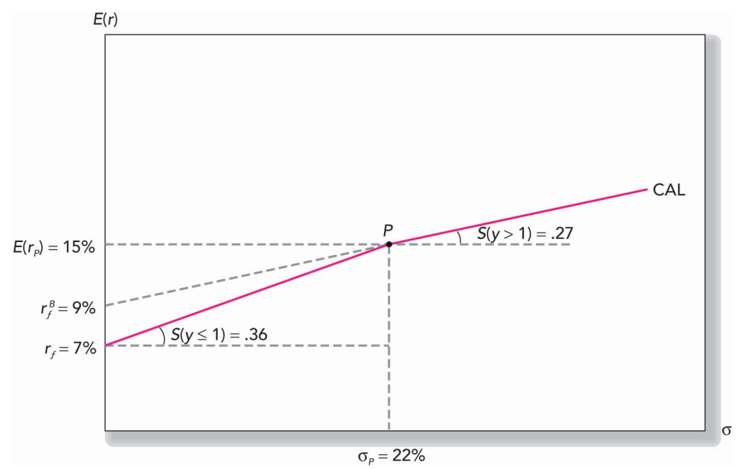
\includegraphics{Resources/capaloocation2.png}

\hypertarget{utility-maximization}{%
\subsection{Utility Maximization}\label{utility-maximization}}

In portfolio theory, investors aim to maximize their utility, which balances expected return and risk. Mathematically, the utility function is:

\[
\begin{aligned}
\text{Max}(U) &= E(r) - \frac{1}{2} A \sigma^2 \\
&= r_f + y [E(r_p) - r_f] - \frac{1}{2} A y^2 \sigma_p^2 \\
\text{Solve for y, we have } \\
y^* &= \frac{E(r_p) - r_f}{A \sigma_p^2}
\end{aligned}
\]

To find the optimal proportion \(y^\) to invest in the risky portfolio, we solve for \(y_*\):

\textbf{R code}

\begin{Shaded}
\begin{Highlighting}[]
\CommentTok{\# Define parameters}
\NormalTok{rf }\OtherTok{\textless{}{-}} \FloatTok{0.06}       \CommentTok{\# Risk{-}free rate}
\NormalTok{Erp }\OtherTok{\textless{}{-}} \FloatTok{0.18}      \CommentTok{\# Expected return of the risky portfolio}
\NormalTok{sigma\_p }\OtherTok{\textless{}{-}} \FloatTok{0.25}  \CommentTok{\# Standard deviation of the risky portfolio}
\NormalTok{A }\OtherTok{\textless{}{-}} \DecValTok{5}           \CommentTok{\# Degree of risk aversion}

\CommentTok{\# Calculate optimal y}
\NormalTok{y\_star }\OtherTok{\textless{}{-}}\NormalTok{ (Erp }\SpecialCharTok{{-}}\NormalTok{ rf) }\SpecialCharTok{/}\NormalTok{ (A }\SpecialCharTok{*}\NormalTok{ sigma\_p}\SpecialCharTok{\^{}}\DecValTok{2}\NormalTok{)}
\NormalTok{y\_star}
\end{Highlighting}
\end{Shaded}

\begin{verbatim}
## [1] 0.384
\end{verbatim}

\begin{Shaded}
\begin{Highlighting}[]
\CommentTok{\# The Expected Return}

\NormalTok{ER }\OtherTok{=}\NormalTok{ rf }\SpecialCharTok{+}\NormalTok{ (y\_star}\SpecialCharTok{*}\NormalTok{(Erp }\SpecialCharTok{{-}}\NormalTok{ rf))}
\NormalTok{ER}
\end{Highlighting}
\end{Shaded}

\begin{verbatim}
## [1] 0.10608
\end{verbatim}

\begin{Shaded}
\begin{Highlighting}[]
\NormalTok{sigma\_c }\OtherTok{=}\NormalTok{ y\_star}\SpecialCharTok{*}\NormalTok{sigma\_p}
\NormalTok{sigma\_c}
\end{Highlighting}
\end{Shaded}

\begin{verbatim}
## [1] 0.096
\end{verbatim}

\begin{Shaded}
\begin{Highlighting}[]
\NormalTok{sharpe }\OtherTok{=}\NormalTok{ (ER}\SpecialCharTok{{-}}\NormalTok{ rf)}\SpecialCharTok{/}\NormalTok{sigma\_c}
\NormalTok{sharpe}
\end{Highlighting}
\end{Shaded}

\begin{verbatim}
## [1] 0.48
\end{verbatim}

\hypertarget{personal-preferences}{%
\subsection{Personal preferences}\label{personal-preferences}}

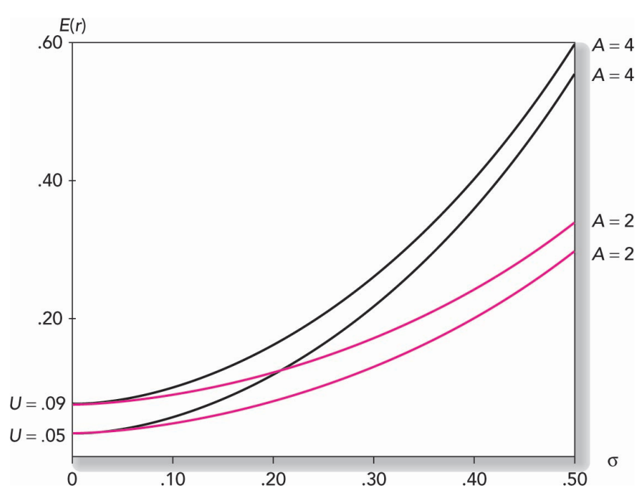
\includegraphics{Resources/capaloocation3.png}

\begin{itemize}
\tightlist
\item
  Investors aim to choose portfolios on higher indifference curves.
\item
  Higher indifference curves provide a higher expected return for a given level of risk.
\item
  More risk-averse investors have steeper indifference curves.
\item
  More risk-averse investors require a greater increase in expected return for an increase in portfolio risk.
\end{itemize}

\hypertarget{the-capital-market-line-cml}{%
\subsection{The Capital Market Line (CML)}\label{the-capital-market-line-cml}}

\begin{longtable}[]{@{}
  >{\raggedright\arraybackslash}p{(\columnwidth - 4\tabcolsep) * \real{0.1829}}
  >{\raggedright\arraybackslash}p{(\columnwidth - 4\tabcolsep) * \real{0.4268}}
  >{\raggedright\arraybackslash}p{(\columnwidth - 4\tabcolsep) * \real{0.3902}}@{}}
\toprule\noalign{}
\begin{minipage}[b]{\linewidth}\raggedright
\textbf{Aspect}
\end{minipage} & \begin{minipage}[b]{\linewidth}\raggedright
\textbf{Active Management}
\end{minipage} & \begin{minipage}[b]{\linewidth}\raggedright
\textbf{Passive Management}
\end{minipage} \\
\midrule\noalign{}
\endhead
\bottomrule\noalign{}
\endlastfoot
\textbf{Pros} & & \\
Higher Return Potential & Aims to outperform the market. & Matches market returns. \\
Flexibility & Can quickly adjust to market changes. & Follows index rules. \\
Risk Management & Can avoid certain sectors or stocks to manage risk. & Diversified holdings reduce specific risks. \\
Exploiting Inefficiencies & Can capitalize on market inefficiencies. & Benefits from overall market growth. \\
Customization & Tailors strategy to investor goals. & Simple, straightforward strategy. \\
\textbf{Cons} & & \\
Higher Costs & More fees and expenses due to frequent trading and research. & Lower fees and expenses. \\
Performance Uncertainty & No guarantee of outperforming the market. & Predictable performance, matches index. \\
Increased Risk & Higher risk from concentrated positions and market timing. & Lower risk due to diversification. \\
Tax Implications & More frequent trading can lead to higher taxes. & Less frequent trading, more tax efficient. \\
Dependence on Manager Skill & Relies on the skill and judgment of the manager. & No reliance on manager skill. \\
\end{longtable}

\hypertarget{ch3}{%
\chapter{Diversification}\label{ch3}}

\begin{itemize}
\item
  calculate mean, variance, and covariance using either historical data or scenario analysis.
\item
  construct efficient portfolios and use the Sharpe ratio to evaluate portfolio efficiency.
\item
  calculate the composition of the optimal risky portfolio.
\end{itemize}

\hypertarget{portfolio-construction-1}{%
\subsection{Portfolio Construction}\label{portfolio-construction-1}}

Portfolio construction generally has three steps:

\begin{enumerate}
\def\labelenumi{\arabic{enumi}.}
\tightlist
\item
  \textbf{Capital allocation} between the risky portfolio and risk-free assets
\item
  \textbf{Asset allocation} across wide asset classes (stocks, international stocks, long-term bonds).
\item
  \textbf{Security selection}.
\end{enumerate}

\hypertarget{major-risks-of-stock-portfolio}{%
\section{Major Risks of Stock Portfolio}\label{major-risks-of-stock-portfolio}}

\begin{longtable}[]{@{}
  >{\raggedright\arraybackslash}p{(\columnwidth - 2\tabcolsep) * \real{0.2687}}
  >{\raggedright\arraybackslash}p{(\columnwidth - 2\tabcolsep) * \real{0.7313}}@{}}
\toprule\noalign{}
\begin{minipage}[b]{\linewidth}\raggedright
Risk Type
\end{minipage} & \begin{minipage}[b]{\linewidth}\raggedright
Description
\end{minipage} \\
\midrule\noalign{}
\endhead
\bottomrule\noalign{}
\endlastfoot
\textbf{Market Risk} & Fluctuations in overall market affecting portfolio value. \\
Sector Risk & Specific sectors or industries under-performing. \\
\textbf{Company Risk} & Individual companies facing financial difficulties or poor performance. \\
Liquidity Risk & Difficulty in buying or selling assets without significant price changes. \\
Currency Risk & Exchange rate fluctuations impacting international investments. \\
Interest Rate Risk & Changes in interest rates affecting bond prices and portfolio value. \\
Political Risk & Political events or policy changes impacting financial markets. \\
Regulatory Risk & Changes in regulations affecting industries or companies in the portfolio. \\
\end{longtable}

\begin{itemize}
\tightlist
\item
  Market risk (\textbf{systematic risk}): non-diversifiable risk
\item
  Unique risk (\textbf{non-systematic risk}): firm-specific risk, diversifiable risk
\end{itemize}

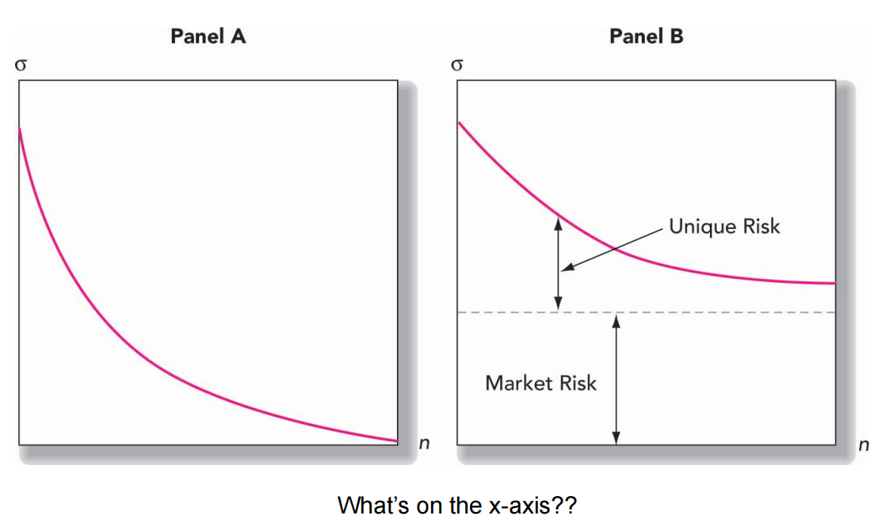
\includegraphics{Resources/sysrisk.png}

\hypertarget{portfolio-calculations}{%
\section{Portfolio Calculations}\label{portfolio-calculations}}

\hypertarget{expected-return-1}{%
\subsection{Expected return}\label{expected-return-1}}

The \textbf{expected return} of the portfolio is

\[ E(r_P) = w_1 E(r_1) + w_2 E(r_2) \]

Where:

\begin{itemize}
\tightlist
\item
  \(E(r_P)\)is the expected return of the portfolio.
\item
  \(w_1\) is the weight of asset 1 in the portfolio.
\item
  \(E(r_1)\) is the expected return of asset 1.
\item
  \(w_2\) is the weight of asset 2 in the portfolio.
\item
  \(E(r_2)\) is the expected return of asset 2.
\end{itemize}

\hypertarget{variance}{%
\subsection{variance}\label{variance}}

\textbf{Variance} measures how much the values of a random variable vary or spread out from the mean (average)

The \textbf{variance} of the portfolio \(\sigma_P^2\) can be calculated using the following formula:

\[ \sigma_P^2 = w_1^2 \sigma_1^2 + w_2^2 \sigma_2^2 + 2w_1 w_2 \rho_{12} \sigma_1 \sigma_2 \]

Where:

\begin{itemize}
\tightlist
\item
  \(\sigma_P^2\) is the variance of the portfolio.
\item
  \(w_1\) is the weight of asset 1 in the portfolio.
\item
  \(\sigma_1^2\) is the variance of returns of asset 1.
\item
  \$w\_2 \$ is the weight of asset 2 in the portfolio.
\item
  \(\sigma_2^2\) is the variance of returns of asset 2.
\item
  \(\rho_{12}\) is the correlation coefficient between returns of assets 1 and 2.
\item
  \(\sigma_1\) and \(\sigma_2\) are the standard deviations of returns of assets 1 and 2, respectively.
\end{itemize}

The variance formula accounts for the individual variances of assets 1 and 2, as well as their \textbf{covariance}.

\[Cov(r_1,r_2 )=\rho_{12} 𝜎_1 𝜎_2\]

\hypertarget{case-i-1}{%
\subsubsection{\texorpdfstring{Case I: \$ \rho = 1 \$}{Case I: \$ = 1 \$}}\label{case-i-1}}

When the correlation coefficient is 1, the formula simplifies to:

\[
\begin{aligned}
\sigma_P^2 &= (w_1 \sigma_1 + w_2 \sigma_2)^2 \\
\sigma_P  &= w_1 \sigma_1 + w_2 \sigma_2 \\
\end{aligned}
\]

\hypertarget{case-ii--1}{%
\subsubsection{\texorpdfstring{Case II: \$ \rho = -1 \$}{Case II: \$ = -1 \$}}\label{case-ii--1}}

When the correlation coefficient is -1, the formula simplifies to:

\[
\begin{aligned}
\sigma_P^2 &= (w_1 \sigma_1 - w_2 \sigma_2)^2 \\
\sigma_P  &= w_1 \sigma_1 - w_2 \sigma_2 \\
\end{aligned}
\]

\hypertarget{covariance}{%
\subsection{Covariance}\label{covariance}}

The \textbf{covariance} between returns of assets A and B (\(Cov(r_A, r_B)\)) can be calculated using the following formula:

\[Cov(r_A, r_B) = \sum_{i=1}^{n} p(i)[r_A(i) - E(r_A)][r_B(i) - E(r_B)]\]

Where:

\begin{itemize}
\tightlist
\item
  \(Cov(r_A, r_B)\) is the covariance between returns of assets A and B.
\item
  \(p(i)\) is the probability of scenario \(i\).
\item
  \(r_A(i)\) and \(r_B(i)\) are the returns of assets A and B, respectively, in scenario \(i\).
\item
  \(E(r_A)\) and \(E(r_B)\) are the expected returns of assets A and B, respectively.
\end{itemize}

\textbf{R code}

\begin{Shaded}
\begin{Highlighting}[]
\NormalTok{returns\_A }\OtherTok{\textless{}{-}} \FunctionTok{c}\NormalTok{(}\FloatTok{0.05}\NormalTok{, }\FloatTok{0.03}\NormalTok{, }\FloatTok{0.02}\NormalTok{, }\FloatTok{0.06}\NormalTok{, }\FloatTok{0.04}\NormalTok{)  }\CommentTok{\# Returns for asset A}
\NormalTok{returns\_B }\OtherTok{\textless{}{-}} \FunctionTok{c}\NormalTok{(}\FloatTok{0.04}\NormalTok{, }\FloatTok{0.02}\NormalTok{, }\FloatTok{0.01}\NormalTok{, }\FloatTok{0.05}\NormalTok{, }\FloatTok{0.03}\NormalTok{)  }\CommentTok{\# Returns for asset B}

\CommentTok{\# Expected returns of assets A and B}
\NormalTok{E\_r\_A }\OtherTok{\textless{}{-}} \FunctionTok{mean}\NormalTok{(returns\_A)}
\NormalTok{E\_r\_B }\OtherTok{\textless{}{-}} \FunctionTok{mean}\NormalTok{(returns\_B)}

\CommentTok{\# Probabilities of scenarios}
\NormalTok{probabilities }\OtherTok{\textless{}{-}} \FunctionTok{c}\NormalTok{(}\FloatTok{0.2}\NormalTok{, }\FloatTok{0.15}\NormalTok{, }\FloatTok{0.25}\NormalTok{, }\FloatTok{0.1}\NormalTok{, }\FloatTok{0.3}\NormalTok{)}

\CommentTok{\# Calculation of covariance}
\NormalTok{covariance }\OtherTok{\textless{}{-}} \FunctionTok{sum}\NormalTok{(probabilities }\SpecialCharTok{*}\NormalTok{ (returns\_A }\SpecialCharTok{{-}}\NormalTok{ E\_r\_A) }\SpecialCharTok{*}\NormalTok{ (returns\_B }\SpecialCharTok{{-}}\NormalTok{ E\_r\_B))}

\CommentTok{\# Print the covariance}
\FunctionTok{print}\NormalTok{(}\FunctionTok{paste}\NormalTok{(}\StringTok{"Covariance between returns of assets A and B:"}\NormalTok{, covariance))}
\end{Highlighting}
\end{Shaded}

\begin{verbatim}
## [1] "Covariance between returns of assets A and B: 0.000175"
\end{verbatim}

\hypertarget{correlation}{%
\subsection{Correlation}\label{correlation}}

\[{\rho_12} = \frac{Cov(r_1,r_2 )}{\sigma_1 \sigma_2}\]

\begin{itemize}
\item
  The portfolio return is not affected by correlation between returns
\item
  Thus, investors should always prefer to add to their portfolios assets with low or negative correlation to diversify risks.
\end{itemize}

The lower the correlation, the greater the potential benefit from diversification.

\hypertarget{variance-calculations}{%
\subsection{Variance calculations}\label{variance-calculations}}

If we have perfectly negatively correlated assets in our portfolios, then the portfolio standard deviation can be reduced to zero by choosing appropriate weights.

Given:

\begin{itemize}
\tightlist
\item
  \(w_1\) = \(0.40\)
\item
  \(\sigma_1^2\) = \(0.014\)
\item
  \(w_2\) = \(0.60\)
\item
  \(\sigma_2^2\) = \(0.04\)
\item
  \(Cov(r_1, r_2)\) = \(0.0072\)
\end{itemize}

Calculate:
\[
\begin{aligned}
\rho        &= \frac{Cov(r_1, r_2)}{\sigma_1 \times \sigma_2} \\ 
            &= \frac{0.007}{\sqrt{0.014} \times \sqrt{0.04}} \\ 
            &= 0.3 \\
\end{aligned}
\]\\
\$\$

\begin{aligned}           
            
 \sigma_P^2 &= w_1^2 \sigma_1^2 + w_2^2 \sigma_2^2 + 2w_1 w_2 \rho(r_1, r_2) \sigma_1 \sigma_2 \\
            &= 0.40^2 (0.014) + 0.60^2 (0.04) + 2(0.40)(0.60)[0.3\sqrt{0.014} \times \sqrt{0.04}] \\
            &= 0.02 \\
\sigma_P    &= \sqrt{0.02} = 0.142 \\
\end{aligned}

\[            
\]

\begin{aligned} 

\text{Weighted}(\sigma) &= 0.40\sqrt{0.014} + 0.60\sqrt{0.04} \\
            &= 0.168 \\
            
\end{aligned}

\$\$

\[
\begin{aligned} 
\text{Diversification Benefit}
            &= 0.168 - 0.142 \\
            &= 0.026 
\end{aligned}
\]

\begin{Shaded}
\begin{Highlighting}[]
\CommentTok{\# Given values}
\NormalTok{w1 }\OtherTok{\textless{}{-}} \FloatTok{0.4}
\NormalTok{w2 }\OtherTok{\textless{}{-}} \FloatTok{0.6}
\NormalTok{sigma1\_squared }\OtherTok{\textless{}{-}} \FloatTok{0.014}
\NormalTok{sigma2\_squared }\OtherTok{\textless{}{-}} \FloatTok{0.04}
\NormalTok{covariance }\OtherTok{\textless{}{-}} \FloatTok{0.0072}

\CommentTok{\# Calculate correlation coefficient}
\NormalTok{rho }\OtherTok{\textless{}{-}}\NormalTok{ covariance }\SpecialCharTok{/} \FunctionTok{sqrt}\NormalTok{(sigma1\_squared }\SpecialCharTok{*}\NormalTok{ sigma2\_squared)}
\NormalTok{rho }
\end{Highlighting}
\end{Shaded}

\begin{verbatim}
## [1] 0.3042555
\end{verbatim}

\begin{Shaded}
\begin{Highlighting}[]
\CommentTok{\# Calculate portfolio variance}
\NormalTok{portfolio\_variance }\OtherTok{\textless{}{-}}\NormalTok{ w1}\SpecialCharTok{\^{}}\DecValTok{2} \SpecialCharTok{*}\NormalTok{ sigma1\_squared }\SpecialCharTok{+}\NormalTok{ w2}\SpecialCharTok{\^{}}\DecValTok{2} \SpecialCharTok{*}\NormalTok{ sigma2\_squared }\SpecialCharTok{+} \DecValTok{2} \SpecialCharTok{*}\NormalTok{ w1 }\SpecialCharTok{*}\NormalTok{ w2 }\SpecialCharTok{*}\NormalTok{ covariance}
\NormalTok{portfolio\_variance}
\end{Highlighting}
\end{Shaded}

\begin{verbatim}
## [1] 0.020096
\end{verbatim}

\begin{Shaded}
\begin{Highlighting}[]
\CommentTok{\# Calculate portfolio standard deviation}
\NormalTok{portfolio\_sd }\OtherTok{\textless{}{-}} \FunctionTok{sqrt}\NormalTok{(portfolio\_variance)}
\NormalTok{portfolio\_sd}
\end{Highlighting}
\end{Shaded}

\begin{verbatim}
## [1] 0.1417604
\end{verbatim}

\begin{Shaded}
\begin{Highlighting}[]
\CommentTok{\# Calculate weighted standard deviation}
\NormalTok{weighted\_sd }\OtherTok{\textless{}{-}}\NormalTok{ w1 }\SpecialCharTok{*} \FunctionTok{sqrt}\NormalTok{(sigma1\_squared) }\SpecialCharTok{+}\NormalTok{ w2 }\SpecialCharTok{*} \FunctionTok{sqrt}\NormalTok{(sigma2\_squared)}
\NormalTok{weighted\_sd}
\end{Highlighting}
\end{Shaded}

\begin{verbatim}
## [1] 0.1673286
\end{verbatim}

\begin{Shaded}
\begin{Highlighting}[]
\CommentTok{\# Calculate diversification benefit}
\NormalTok{diversification\_benefit }\OtherTok{\textless{}{-}}\NormalTok{ weighted\_sd }\SpecialCharTok{{-}}\NormalTok{ portfolio\_sd}
\NormalTok{diversification\_benefit}
\end{Highlighting}
\end{Shaded}

\begin{verbatim}
## [1] 0.02556828
\end{verbatim}

\hypertarget{risky-and-risk-free-assets}{%
\section{Risky and Risk-Free Assets}\label{risky-and-risk-free-assets}}

To decide the proportion of the portfolio to be allocated between the stock and bond funds, we will introduce a risk-free asset (T-bills) to the portfolio allocation problem.

\hypertarget{sharpe-ratio}{%
\subsection{Sharpe Ratio}\label{sharpe-ratio}}

The higher a fund's Sharpe ratio (Higher Return per Unit of Risk), the better its returns have been relative to the amount of investment risk taken.

\begin{longtable}[]{@{}ll@{}}
\toprule\noalign{}
Sharpe Ratio Range & Classification \\
\midrule\noalign{}
\endhead
\bottomrule\noalign{}
\endlastfoot
Less than 1 & Bad \\
1 to 1.99 & Adequate/Good \\
2 to 2.99 & Very Good \\
\end{longtable}

The objective function is to maximize:

\[\frac{{E(r_1) - r_f}}{{\sigma_P}}\]

where:

\[
\begin{aligned} 
E(r_1)    &= w_1 E(r_1) + w_2 E(r_2)\\
\sigma_P  &= \sqrt{{w_1^2 \sigma_1^2 + w_2^2 \sigma_2^2 + 2w_1 w_2 Cov(r_1, r_2)}}\\
\text{subject to}:\\
w_1 + w_2 &= 1\\
\end{aligned} 
\]

\hypertarget{optimal-complete-portfolio}{%
\subsection{Optimal Complete Portfolio}\label{optimal-complete-portfolio}}

\hypertarget{the-efficient-frontier}{%
\subsection{The Efficient Frontier}\label{the-efficient-frontier}}

\hypertarget{separation-property}{%
\subsection{Separation Property}\label{separation-property}}

\hypertarget{ch4}{%
\chapter{CAPM and APT}\label{ch4}}

\hypertarget{enter-subsection-1-here}{%
\section{Enter subsection 1 here}\label{enter-subsection-1-here}}

\hypertarget{enter-subsection-2-here}{%
\section{Enter subsection 2 here}\label{enter-subsection-2-here}}

\hypertarget{ch5}{%
\chapter{Enter Chapter title here}\label{ch5}}

\hypertarget{enter-subsection-1-here-1}{%
\section{Enter subsection 1 here}\label{enter-subsection-1-here-1}}

\hypertarget{enter-subsection-2-here-1}{%
\section{Enter subsection 2 here}\label{enter-subsection-2-here-1}}

\hypertarget{ch6}{%
\chapter{Enter Chapter title here}\label{ch6}}

\hypertarget{enter-subsection-1-here-2}{%
\section{Enter subsection 1 here}\label{enter-subsection-1-here-2}}

\hypertarget{enter-subsection-2-here-2}{%
\section{Enter subsection 2 here}\label{enter-subsection-2-here-2}}

\hypertarget{ch7}{%
\chapter{Enter Chapter title here}\label{ch7}}

\hypertarget{enter-subsection-1-here-3}{%
\section{Enter subsection 1 here}\label{enter-subsection-1-here-3}}

\hypertarget{enter-subsection-2-here-3}{%
\section{Enter subsection 2 here}\label{enter-subsection-2-here-3}}

\hypertarget{ch8}{%
\chapter{Performance Attribution and Appraisal}\label{ch8}}

\hypertarget{enter-subsection-1-here-4}{%
\section{Enter subsection 1 here}\label{enter-subsection-1-here-4}}

\hypertarget{enter-subsection-2-here-4}{%
\section{Enter subsection 2 here}\label{enter-subsection-2-here-4}}

\hypertarget{ch9}{%
\chapter{Tax Implications and ESG Investing}\label{ch9}}

\hypertarget{enter-subsection-1-here-5}{%
\section{Enter subsection 1 here}\label{enter-subsection-1-here-5}}

\hypertarget{enter-subsection-2-here-5}{%
\section{Enter subsection 2 here}\label{enter-subsection-2-here-5}}

\hypertarget{concluding-remarks}{%
\chapter*{Concluding Remarks}\label{concluding-remarks}}
\addcontentsline{toc}{chapter}{Concluding Remarks}

\hypertarget{three-points-learnt}{%
\section*{Three points learnt}\label{three-points-learnt}}
\addcontentsline{toc}{section}{Three points learnt}

Summarise three major point that you learnt from this course:

\begin{itemize}
\tightlist
\item
\item
\item
\end{itemize}

\hypertarget{three-questions-to-ask}{%
\section*{Three questions to ask}\label{three-questions-to-ask}}
\addcontentsline{toc}{section}{Three questions to ask}

Come up with three questions to ponder:

\begin{itemize}
\tightlist
\item
\item
\item
\end{itemize}

\hypertarget{remarks}{%
\section*{Remarks}\label{remarks}}
\addcontentsline{toc}{section}{Remarks}

\begin{itemize}
\tightlist
\item
\end{itemize}

\hypertarget{how-to-use-rbookdown}{%
\chapter*{How to use RBookDown}\label{how-to-use-rbookdown}}
\addcontentsline{toc}{chapter}{How to use RBookDown}

Firstly, you will have to read the \href{https://bookdown.org/yihui/bookdown/}{RBookDown Bible} by YiHui Xie

In essence, you write in a mixture of markdown (For basics), html (to extend on markdown) and latex language (mostly for equations) to create a simple Note.

You can customise your style and theme through your own CSS.

RMarkdown are mostly used to knit e-books(HTML), use TexStudio if you want a proper PDF, it is easier.

\textbf{Here are some useful tips to get started}

1: To add a chapter, just open a R file and save as \texttt{.RMD}. Use number 0 to 99 with a hyphen \texttt{-} to order the RMD files and maybe add a Chapter name so it is easier to select from \texttt{Files} window at bottom right of the R Studio.

2: Code chunks can generate graphical outputs, To insert pictures just use \texttt{include\_graphics} instead of \texttt{\textbackslash{}includegraphics\{\}} or \texttt{!{[}{]}()}. Width can be customised.

\begin{verbatim}
knitr::include_graphics(rep('images/knit-logo.png', 3))
\end{verbatim}

3: Use 1 grave accent ` to include the in line code, use 3 grave accent to include a chunk of code.

  \bibliography{references.bib}

\end{document}
